\subsection{Useful accepted work, prices and complete costs}

The answer is positive within the declared model: competent Beta delivers useful accepted coordination-design work, collects customer payments, covers complete delivery and business costs, and leaves operating surplus. It needs no graph advantage or separate R\&D to meet that commercial criterion. The outcome remains conditional on task performance, human-scope equivalence, buyer demand and workload assumptions; it is not realized revenue.

Customers receive an executable bounded coordination mechanism, task-specific checks and counterexamples, declared assumptions, integration artifacts and a handoff. They do not buy an untested idea or an operational market guarantee. The three human-service references are USD25,329, USD49,857.64 and USD98,114.56 for assumed teams of 100, 196 and 384 hours, using the documented US rates in Table~\ref{tab:human}. They are derived matched-scope scenarios, not actual customer quotations or verified human-only labor.

\begin{table}[H]\centering\small\caption{Commercial core: Beta-only means over 64 fresh worlds per scenario. USD unless noted; 104 intake weeks plus 16 run-off weeks.}\label{tab:commercial}

\begin{tabular}{lrrr}\toprule Metric & Conservative & Central & Favorable\\\midrule

Useful accepted outcomes & 48.39 & 163.00 & 208.36 \\

Price / human reference & 29.8\% adaptive & 55\% fixed & 75\% fixed \\

Mean completed-job quote & 13,960 & 25,844 & 35,075 \\

Collected receipts & 677,921 & 4,192,972 & 7,377,908 \\

A: full delivery expenses & 209,756 & 432,391 & 556,141 \\

Common setup and business costs & 56,744 & 57,715 & 58,288 \\

Closing obligations & 0 & 471 & 0 \\

\textbf{Collected operating profit} & 411,421 & 3,702,395 & 6,763,479 \\

Available closing cash & 470,952 & 3,761,488 & 6,821,122 \\

\textbf{Buffered surplus above seed} & 408,312 & 3,698,570 & 6,758,482 \\

\bottomrule\end{tabular}\end{table}

B and C expenses are zero in these Beta arms. A includes learning during delivery, failed work, tools, verification, correction, packaging, refunds and recovery. Common costs include the USD9,500 bootstrap and shared business infrastructure. Initial USD60,000 capital is not revenue or profit. The central closing-obligation mean is deducted conservatively; already-accrued unpaid expense is not deducted twice.

The policy search used buyer choices among our offer, a human service, postponement and no purchase. These prices were selected in the declared 32-policy network family before confirmation and then applied unchanged to Beta. They are evaluated, economically selected policies, not an independent proof of the globally best Beta price. Conservative realized offer ratios range from 25\% to 45\%; central and favorable fixed ratios are 55\% and 75\%. A lower price alone does not establish real demand.

\subsection{Surplus, usable cash and correct-outcome receipts}

Available cash removes the ledger's protected commitments, warranty reserves and unpaid expenses. It is different from profit and includes seed. The final table row is a reporting-only planning measure: $\max(0,\min(\Pi,\text{available cash}-60{,}000)-2{,}640)$. It preserves initial seed, caps the figure by reported profit, and leaves a six-week Beta operating buffer. The USD2,640 buffer is not another expense or a claim that all future liabilities are known.

\begin{figure}[H]\centering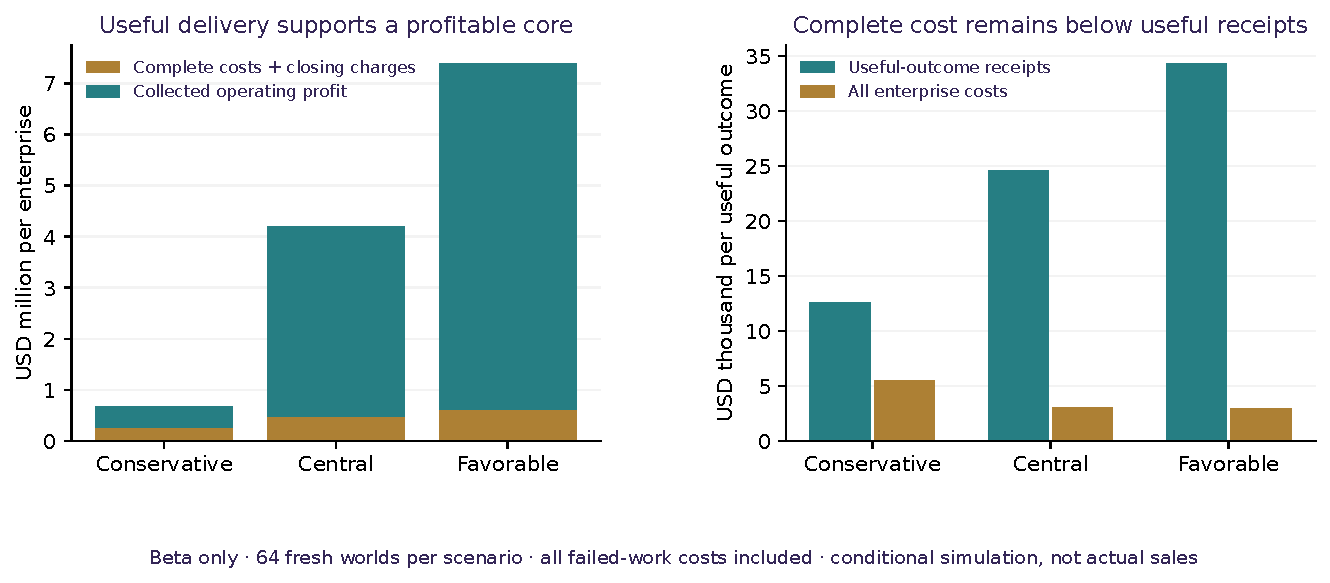
\includegraphics[width=\linewidth]{figures/commercial.pdf}\caption{The commercial core before optional skills. All quantities are modeled; every cost of failed work remains in the accounting.}\end{figure}

To avoid crediting the commercial conclusion to erroneous deliveries, a retrospective accounting check keeps only receipts linked to on-time, truly correct outcomes and still deducts every enterprise expense and unexpensed closing obligation, including refunds and recovery of incorrect work. This is a deliberately conservative cash-revenue sensitivity, not a newly tuned policy or another sample.

\begin{table}[H]\centering\small\caption{Commercial checks using only useful-outcome receipts. Pooled per-outcome ratios use the same useful-outcome denominator.}

\begin{tabular}{lrrr}\toprule Metric & Conservative & Central & Favorable\\\midrule

Useful receipts per useful outcome & 12,604 & 24,622 & 34,279 \\

All costs per useful outcome & 5,507 & 3,010 & 2,949 \\

Conservative surplus per useful outcome & 7,097 & 21,612 & 31,330 \\

Useful-receipt-only total surplus & 343,435 & 3,522,731 & 6,527,982 \\

Worst world in this check & -30,129 & 1,517,350 & 2,826,354 \\

\bottomrule\end{tabular}\end{table}

Mean surplus remains positive in every scenario under that stricter check: USD343,435, USD3,522,731 and USD6,527,982. The conservative minimum is USD$-30,128.78$, so the result is not a guarantee that every world remains profitable under every accounting sensitivity. Pooled ratios summarize a heterogeneous portfolio; they are not a matched-job quote or an empirical productivity multiple.

The modeled customer savings on useful outcomes average USD1.67, USD3.43 and USD2.43 million across the three scenarios relative to their declared human references. These are price differences for supported useful outcomes, not measured consumer welfare, willingness to pay or evidence of actual sales. Quality is a simulated latent property. Positive economics cannot certify a real professional service or a real minimum quality floor.

\subsection{Throughput, capital and commercial downside}

The six-producer, two-validator configuration supports mean useful throughput of 0.47, 1.57, 2.00 outcomes per intake week, respectively. Dividing by the full 120-week horizon gives lower rates; neither measure is observed production or a steady-state capacity guarantee. The primary scenarios assume 1.8, 4 and 7 initial qualified leads per week, with repeat demand modeled separately.

The primary runs begin with USD60,000 and collect after seven, four and two weeks in the three scenarios. They record no Beta cash shortfall in 64 worlds each; the Wilson 95\% upper bound is nevertheless 5.66\%. A dedicated central-prior stress fails in all 16 worlds at USD10,000 seed and has zero observed shortfalls at USD25,000. This brackets tested outcomes, not an identified minimum required capital or a guarantee at USD25,000.

Demand sensitivity brackets the mean-profit crossing between 0.05 and 0.25 initial qualified leads per week at the frozen central price and other assumptions. Reducing the human reference to 10\% leaves positive mean Beta surplus of about USD80,204, while the combined low-demand, low-reference, high-cost, low-trust and slow-collection case loses about USD16,661. Thus the commercial core has explicit failure conditions even though the three primary scenario means are positive.

A split-sample capacity menu selects doubling producers, validators and quotas together. Its eight fresh test worlds improve Beta mean surplus by USD1,331,416, with conditional Monte Carlo interval [USD685,519, USD1,977,314], after the modeled capacity costs. That resource decision does not depend on skill sharing. It tests an initial capacity choice, not global optimal expansion timing. Spending still requires currently available cash.

These findings support continued modeled Beta delivery and retained reserves as economically meaningful choices. The next sections ask whether a candidate skill, sharing policy or extra investment adds enough value to improve that already-profitable foundation. Optional enhancements are allowed to fail their own tests without discarding the commercial core.
